\section*{Anexo C. Fase exploratoria}
\phantomsection
\addcontentsline{toc}{subsection}{Anexo C. Fase exploratoria}
\setcounter{table}{0}
\renewcommand{\thetable}{C.\arabic{table}}
\renewcommand{\theHtable}{C.\arabic{table}}
\setcounter{figure}{0}
\renewcommand{\thefigure}{C.\arabic{figure}}
\renewcommand{\theHfigure}{C.\arabic{figure}}

Antes del plan de pruebas hubo una fase exploratoria en la que se
construyeron y probaron los módulos U2, U3 y U4 sobre escenarios
sintéticos. Este anexo la registra de forma condensada. Sus
conclusiones las reemplaza el plan de pruebas
(Capítulo~\ref{cap:resultados}). Se conservan porque explican las
decisiones que llevaron al plan y porque dos pruebas de esta fase, el
agente tabular con cuatro fases y el canal de mensajes imperfecto, no se
repitieron en él.

El protocolo de esta fase difiere del plan en cuatro puntos. La
evaluación final usaba diez semillas (1001 a 1010). Q-learning se
entrenaba con la recompensa de colas (Ecuación~\ref{eq:recompensa}),
una sola semilla base y entre 40 y 120 episodios, con $\varepsilon$
multiplicado por 0.9 al terminar cada episodio hasta un piso de 0.05
(por 0.96 en cruce2 y por 0.95 en red). Q-learning e IPPO publicaban la
política del último episodio, sin elegir un \textit{checkpoint} por
validación. Y los programas fijos se tunearon en parte con semillas de
evaluación.
% fuente: episodios y decaimiento de epsilon, columna epsilon de resultados_<esc>.csv de demo_rl
% (cruce, corredor y corredor_alta: 40 episodios con 0.9; cruce2: 120 con 0.96; red: 100 con 0.95)

IPPO, en cambio, ya usaba la recompensa de retraso
(Ecuación~\ref{eq:recompensa-u4}) y tres semillas base de 200
episodios. De sus tres políticas se cita la mediana según la evaluación
intermedia final, que es la de la política congelada con la sola
semilla 999.

Esta fase y el resultado principal del plan miden el retraso con la
misma métrica, el \texttt{timeLoss} de SUMO, pero frente a programas
fijos distintos. Por eso sus cifras no se comparan directamente con las
del Capítulo~\ref{cap:resultados}. Cuando este anexo cita el plan de
pruebas, usa su resultado principal
en P1 a P6, y lo que compara con esta
fase es el signo y el orden de
magnitud. El análisis de robustez del plan (Sección~\ref{sec:robustez})
repite la comparación con el retraso total, que suma la espera para
entrar a la red, y con un fijo re-barrido hasta verdes de 10~s. En P2 y
P3, dos de los casos que se citan aquí, esa comparación cambia la
lectura, y el anexo lo indica donde corresponde.
% fuente: evaluacion_<esc>_resumen.csv de demo_rl (fase exploratoria, timeloss_prom); resultado principal:
% plan2/veredicto.csv de la corrida principal (= plan2/veredicto_congelado_0355.csv en P1-P5);
% robustez: plan2/robustez_veredicto.csv y hechos_v21.md

Los casos se numeran con la letra E:
E1 (cruce), E2 (cruce2), E3 (corredor) y E4 (red) para el agente
tabular; E3-U4 y E4-U4 para IPPO en corredor y red; y E6 para
corredor\_alta. Corredor, corredor\_alta y red son los escenarios de P1,
P2 y P3 (Tabla~\ref{tab:plan2-casos}); cruce y cruce2 no son casos del
plan, y cruce se usa además en las pruebas de humo
(Sección~\ref{sec:humo}).

\subsection*{Escenarios cruce y cruce2}

El escenario cruce es una intersección aislada de dos ejes, N--S y
E--O, con un carril por sentido y dos fases verdes. En la punta el eje
principal lleva 650~veh/h por sentido, la transversal 150 y los giros
entre 40 y 80 (1844 vehículos en la hora); su programa fijo da 25~s de
verde por fase, con ciclo de 56~s. El escenario cruce2 tiene dos
carriles por sentido, un carril exclusivo de giro a la izquierda y
cuatro fases verdes, dos de ellas de giro protegido. En la punta lleva
420~veh/h por sentido en los movimientos rectos, 160 en el giro a la
izquierda y 200 en la transversal (1884 vehículos); su fijo da 20~s a
las fases principales y 6~s a las de giro, con ciclo de 64~s. Ambos
usan el vehículo, el ámbar de 3~s y la demanda con punta invertida de
los casos del plan (Sección~\ref{sec:escenarios}).
% fuente: filas cruce y cruce2 de tab:escenarios en el texto original
% (git show 7bd8685:TESIS/secciones/capitulo4.tex, l.434-435)

\subsection*{Programa fijo de referencia}

El programa fijo se ajustó en dos rondas. La primera barría un solo
verde común a todas las aproximaciones y, en los corredores, el
desfase. El criterio fue primero la espera detenida y después el
retraso, sobre las semillas 1001 a 1003, que forman parte de las de
evaluación (\texttt{barrer\_fijo.py}, Anexo~B). Nunca variaba el
reparto entre la avenida y las transversales, aunque la avenida lleva entre tres y cinco
veces más demanda. La segunda ronda barrió el reparto y el desfase sobre
las semillas 2001 a 2003, con el verde transversal acotado por abajo a
los 10~s del verde mínimo del agente, en cruce, corredor, red y
corredor\_alta. Las comparaciones de este anexo usan esos fijos.

En cruce el reparto original de 25/25 (verde de la avenida/verde
transversal, en segundos) resultó el mejor de las 36 combinaciones,
porque la punta cambia de eje a mitad de hora y ningún reparto fijo
favorece a los dos periodos. En corredor el reparto
sí importaba: 20~s para la avenida, 10~s para las transversales y
desfase de 15~s dan 21.2~s de retraso sobre las semillas de evaluación,
frente a 31.9~s del 25/25 con desfase de 25~s de la primera ronda. En
red el reparto pasó de 20/20 a 25/15 con los mismos desfases y el
retraso bajó de 22.2 a 21.8~s.

El fijo de cruce2 es el de la primera ronda. El reparto sin ajustar lo
debilita y las semillas compartidas lo favorecen, y ninguno de los dos
defectos alcanza para invertir el margen de $+17$\,\% con que pierde el
agente tabular.

\subsection*{Q-learning con la recompensa de colas}

La Tabla~\ref{tab:resumen-escenarios} reúne la métrica primaria de los
cuatro escenarios nominales; en ella, RL designa al Q-learning con la
recompensa de colas. El agente reduce el retraso frente al fijo solo en
el cruce de dos fases ($-6$\,\%) y lo aumenta en los otros tres:
$+15$\,\% en red, $+17$\,\% en cruce2 y $+60$\,\% en corredor. En
ningún caso alcanza la meta de $-25$\,\%. El actuado, con los mismos
límites de verde que el agente, mejora al fijo en tres escenarios (de
$-2$\,\% en red a $-33$\,\% en cruce), empata con el del corredor y es
mejor que el agente en los cuatro.

% Generado por tablas_tex.py a partir de los CSV del proyecto. No editar a mano.
\begin{table}[H]
\setstretch{1}
\centering
\scriptsize
\setlength{\tabcolsep}{3pt}
\begin{tabular}{lrrrrrrrr}
\toprule
 & \multicolumn{3}{c}{Retraso (s/veh)} & \multicolumn{2}{c}{RL vs fijo} & Actuado & \multicolumn{2}{c}{RL vs fijo, secundarias} \\
\cmidrule(lr){2-4}\cmidrule(lr){5-6}\cmidrule(lr){7-7}\cmidrule(lr){8-9}
Escenario & Fijo & Actuado & RL & $\Delta$ [IC95\,\%] & $p$ & $\Delta$ vs fijo & Espera & Paradas \\
\midrule
cruce & 23.19 & 15.46 & 21.72 & $-$6.4\,\% [$-$9.3, $-$2.7] & 0.0137 & $-$33.4\,\% & $-$25.9\,\% & +27.4\,\% \\
cruce2 & 27.54 & 23.21 & 32.15 & +16.7\,\% [9.9, 25.4] & 0.00195 & $-$15.7\,\% & +18.4\,\% & +23.5\,\% \\
corredor & 21.15 & 20.91 & 33.86 & +60.1\,\% [53.2, 66.9] & 0.00195 & $-$1.1\,\% & +75.9\,\% & +93.6\,\% \\
red & 21.78 & 21.42 & 25.12 & +15.3\,\% [13.9, 16.8] & 0.00195 & $-$1.7\,\% & +4.0\,\% & +75.6\,\% \\
\bottomrule
\end{tabular}
\caption[Resumen por escenario]{Resumen por escenario: retraso promedio por vehículo con política congelada, 10 semillas de evaluación comunes a los tres controles. La meta de la tesis es $-25$\,\% de retraso frente al fijo.}
\label{tab:resumen-escenarios}
\end{table}


\subsection*{E1: cruce de dos fases}

En el cruce la tabla Q termina con 130 estados visitados de 512
posibles tras 40 episodios. Con la política congelada el agente reduce
el retraso un $6.4$\,\% frente al fijo (intervalo $-9.3$ a $-2.7$\,\%,
$p = 0.014$) y la espera detenida un $26$\,\%, pero aumenta las paradas
por vehículo un $27$\,\% (Tablas~\ref{tab:resumen-escenarios}
y~\ref{tab:cruce-u4}). Cambia de fase 233
veces por hora frente a 131 del fijo, porque corta el verde en cuanto
la cola del eje en rojo supera a la del eje en verde. Eso acorta las
esperas pero obliga a más vehículos a frenar y volver a arrancar, y el
retraso, que incluye esas maniobras, mejora mucho menos que la espera.
El actuado reduce el retraso un $33$\,\%.

\subsection*{E2: cruce con giros protegidos}

Con cuatro fases verdes el espacio de estados crece a 1024. Con
decaimiento de 0.96 y 120 episodios, la tabla Q termina con 390
estados (Figura~\ref{fig:cruce2-qtable}): más de la mitad del espacio
nunca se visitó, y en los estados poco visitados la política
\textit{greedy} elige entre valores apenas actualizados. La política
congelada queda por encima del fijo en 14 de las 24 evaluaciones
intermedias, y en cinco de ellas (episodios 5, 10, 60, 75 y 120) se
bloquea, con retrasos de entre 47 y 210~s.

\begin{figure}[H]
  \centering
  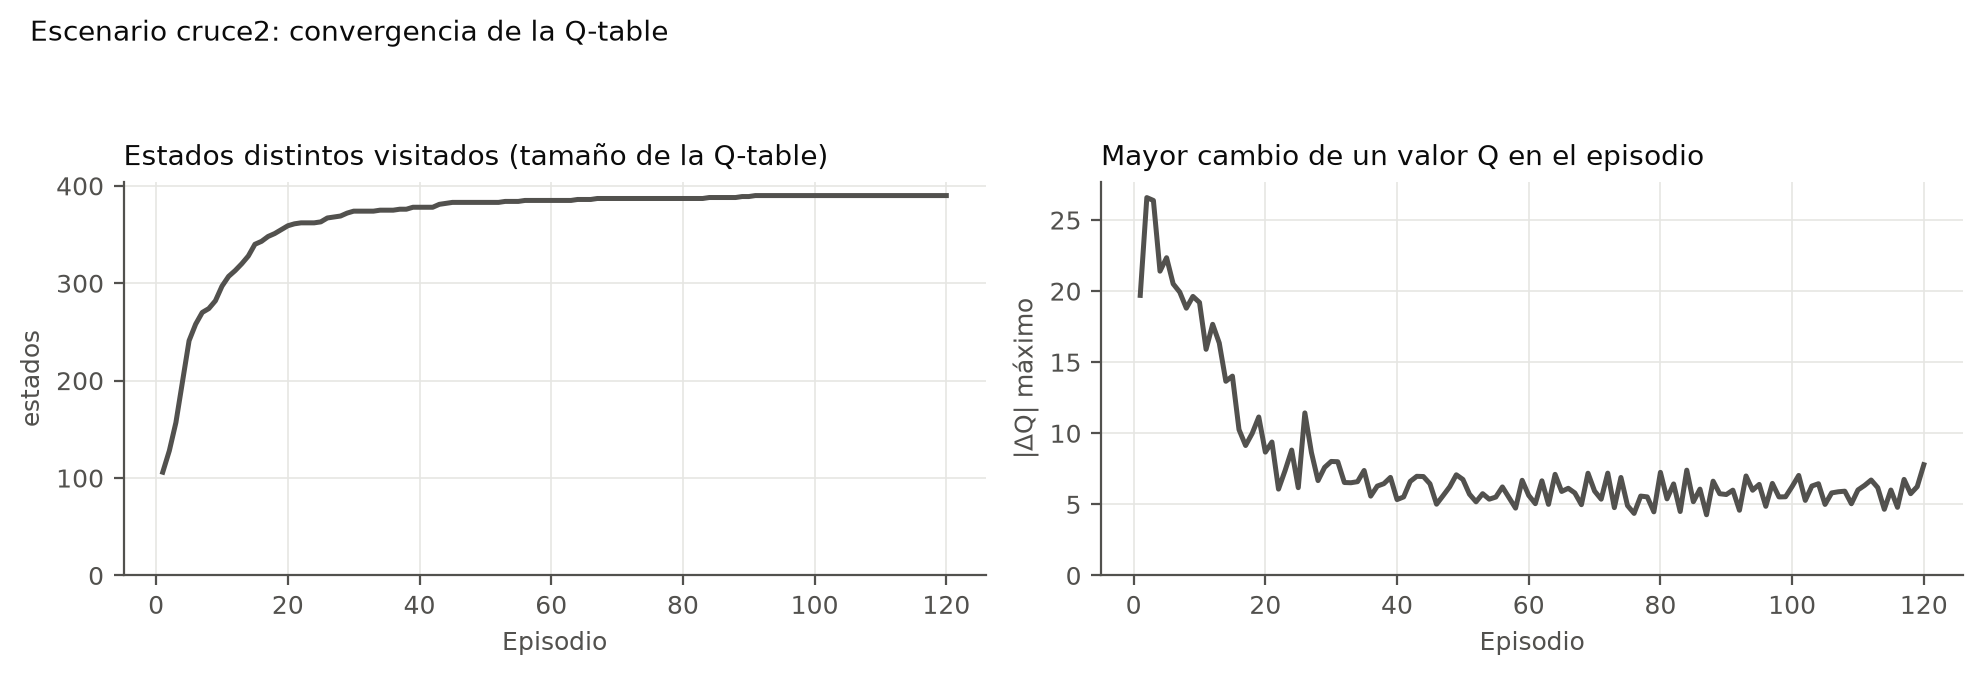
\includegraphics[width=\textwidth]{fig_cruce2_qtable.png}
  \caption[Escenario cruce2: cobertura de la tabla Q]{Escenario cruce2 (fase exploratoria): estados distintos visitados por la tabla Q en cada uno de los 120 episodios de entrenamiento (390 de 1024 posibles al terminar) y mayor cambio de un valor Q en el episodio.}
  \label{fig:cruce2-qtable}
\end{figure}

En la evaluación final (Tabla~\ref{tab:cruce2-evaluacion}) el agente es
peor que el fijo en retraso, espera, colas, paradas y emisiones. El
retraso sube un $17$\,\% (intervalo $+10$ a $+25$\,\%, $p = 0.002$), con
una desviación estándar entre semillas unas diecinueve veces la del fijo
(3.7 frente a 0.2~s), mientras el actuado lo reduce un $16$\,\%.

Es el argumento empírico para pasar a la aproximación de funciones: la tabla
no cubre el espacio de estados cuando hay fases de giro protegido, y
más episodios no lo resuelven. Ningún caso ejecutado del plan tiene giro
protegido (P7 queda como trabajo siguiente), así que este resultado no
tiene contraparte en el Capítulo~\ref{cap:resultados}.

% Generado por tablas_tex.py a partir de los CSV del proyecto. No editar a mano.
\begin{table}[H]
\setstretch{1}
\centering
\scriptsize
\setlength{\tabcolsep}{3pt}
\setlength{\tabcolsep}{2pt}
\begin{tabular}{lrrrrrr}
\toprule
Métrica & Tiempo fijo & Actuado & Q-learning & \makecell{$\Delta$ RL vs fijo\\{}[IC95\,\%]} & $p$ & \makecell{$\Delta$ actuado\\vs fijo} \\
\midrule
Retraso (s/veh) & 27.54 $\pm$ 0.14 & 23.21 $\pm$ 0.15 & 32.15 $\pm$ 2.63 & \makecell{+16.7\,\%\\{}[9.9, 25.4]} & 0.00195 & $-$15.7\,\% \\
Espera detenida (s/veh) & 15.63 $\pm$ 0.12 & 11.69 $\pm$ 0.14 & 18.51 $\pm$ 1.77 & \makecell{+18.4\,\%\\{}[10.2, 28.7]} & 0.00195 & $-$25.2\,\% \\
Cola promedio (veh) & 7.49 $\pm$ 0.07 & 5.75 $\pm$ 0.06 & 9.21 $\pm$ 0.91 & \makecell{+23.0\,\%\\{}[14.3, 34.0]} & 0.00195 & $-$23.3\,\% \\
Cola máxima (veh) & 22.50 $\pm$ 0.51 & 17.90 $\pm$ 0.63 & 29.90 $\pm$ 4.31 & \makecell{+32.9\,\%\\{}[19.1, 50.9]} & 0.00195 & $-$20.4\,\% \\
Paradas por vehículo & 0.88 $\pm$ 0.01 & 0.84 $\pm$ 0.01 & 1.08 $\pm$ 0.08 & \makecell{+23.5\,\%\\{}[17.5, 31.2]} & 0.00195 & $-$4.1\,\% \\
Throughput (veh) & 1840.60 $\pm$ 0.69 & 1844.40 $\pm$ 0.91 & 1842.50 $\pm$ 0.84 & \makecell{+0.1\,\%\\{}[0.0, 0.2]} & 0.0156 & +0.2\,\% \\
Recompensa por decisión & $-$8.13 $\pm$ 0.07 & $-$6.00 $\pm$ 0.07 & $-$10.04 $\pm$ 1.02 & \makecell{+23.6\,\%\\{}[14.5, 35.1]} & 0.00195 & $-$26.2\,\% \\
Cambios de fase & 230.80 $\pm$ 0.74 & 288.30 $\pm$ 2.34 & 280.80 $\pm$ 2.07 & \makecell{+21.7\,\%\\{}[20.9, 22.4]} & 0.00195 & +24.9\,\% \\
\bottomrule
\end{tabular}
\caption[Escenario cruce2: evaluación con política congelada]{Escenario cruce2: evaluación con política congelada sobre 10 semillas (1001 a 1010), las mismas para los tres controles. Media $\pm$ IC95\,\%; el cambio porcentual lleva su intervalo bootstrap pareado y $p$ es el de la prueba de Wilcoxon pareada frente al fijo.}
\label{tab:cruce2-evaluacion}
\end{table}


\subsection*{E3: corredor de dos cruces}

En el corredor cada cruce tiene su propio agente, sin comunicación
entre ellos. Frente al fijo tuneado, que da $21.2 \pm 0.4$~s, los dos
agentes aumentan el retraso un $60$\,\% (intervalo $+53$ a $+67$\,\%,
$p = 0.002$; Tablas~\ref{tab:resumen-escenarios}
y~\ref{tab:corredor-u4}). Frente al fijo de la primera
ronda perdían solo un $6$\,\% y reducían la espera un $13$\,\%: la
magnitud de la derrota depende de lo bien tuneada que esté la
referencia. El actuado, que tampoco coordina, empata con el fijo
tuneado ($-1.1$\,\%, intervalo $-2.5$ a $+0.5$\,\%).

El plan de pruebas corrigió esa magnitud, pero no el signo. En P1,
sobre el mismo corredor, con la misma recompensa de colas y el
protocolo del plan, la pérdida frente al fijo es del $10.6$\,\%, y con
la recompensa de retraso, del $9.2$\,\%. Casi toda la corrección viene
del protocolo: en esta fase había una sola semilla base, 40 episodios y
la política del último episodio.
% fuente: plan2/veredicto_congelado_0355.csv (P1, ql y ql_colas, delta_fijo); texto original
% (git show 7bd8685:TESIS/secciones/conclusiones.tex, conclusiones 4 y 7)

La política tabular es además frágil. Una corrida previa del mismo
caso, con un desfase del reloj de decisión que dejaba el verde mínimo
efectivo en 12~s en vez de 10, dio 25.8~s; con la restricción corregida
la política da 33.9~s. Esa diferencia de 8~s es unas cinco veces la
semiamplitud del intervalo de confianza de la política (1.7~s): la
varianza entre entrenamientos no es pequeña, y por eso el módulo U4
entrenó tres políticas por variante.
% fuente: evaluacion_corredor_resumen.csv de demo_rl (brazo rl, timeloss_prom: media 33.856, ic95 1.661)

\subsection*{E4: red de tres cruces con onda verde}

En la red el fijo es una onda verde: 25~s para la avenida, 15~s para
las transversales y desfases de 0, 23 y 0~s (23~s es el tiempo de
viaje entre cruces; ciclo de 46~s), con $21.8 \pm 0.2$~s de retraso. Los
tres agentes quedan un $15$\,\% por encima (intervalo $+14$ a
$+17$\,\%, $p = 0.002$; Tablas~\ref{tab:resumen-escenarios}
y~\ref{tab:red-u4}). No es falta de
entrenamiento: con 100 episodios la evaluación intermedia se mantiene
entre 23.8 y 25.5~s desde el episodio~5, sin tendencia a bajar. Tampoco
son malos en términos absolutos: el mismo fijo sin desfases da
$36.4 \pm 0.2$~s, frente a 25.1~s del agente.

Lo que los agentes no consiguen es reproducir la progresión de la onda
verde: cada uno reacciona a su cola local y la rompe. El actuado, que
tampoco coordina, apenas mejora al fijo ($-2$\,\%). Este resultado
motivó el módulo U4: con varios semáforos consecutivos, la coordinación
anticipada vale más que la reacción local.

\subsection*{Lectura del agente tabular}

En cruce y red la espera detenida, que es la señal de la recompensa de
colas, sale mejor parada que el retraso: en cruce baja un $26$\,\%
mientras el retraso baja un $6$\,\%, y en red sube un $4$\,\% mientras
el retraso sube un $15$\,\%. En cruce2 y corredor empeoran las dos. La
diferencia son las paradas adicionales de un agente que cambia de fase
entre un $13$ y un $77$\,\% más veces que el fijo; las paradas por
vehículo suben en los cuatro escenarios.

El plan de pruebas confirmó el signo en corredor y red, con una pérdida
mucho menor en el corredor (E3), y aisló el efecto de la recompensa:
Q-learning con la recompensa de retraso falla en P1 y P3 ($+9.2$ y
$+12.4$\,\% frente al fijo), igual que la ablación \texttt{ql\_colas},
que conserva la recompensa de colas ($+10.6$ y $+9.6$\,\%). Con demanda
nominal o moderada el cambio de recompensa mueve el resultado menos de
tres puntos, y el techo tabular no se explica por ella. Solo en P2 la
recompensa de retraso cambia el signo: $-8.8$\,\% frente a $+6.8$\,\%
con la de colas, este último provisional porque no convergió
(Anexo~A). Esa mejora de Q-learning en P2 no resiste el análisis de
robustez: su espera para entrar a la red es de 357~s/veh, frente a 240
del fijo, y con el retraso total queda un $26.4$\,\% por encima del
fijo (Sección~\ref{sec:robustez}).
% fuente: plan2/veredicto_congelado_0355.csv, filas ql y ql_colas de P1 a P4 (columnas delta_fijo y
% veredicto; ql_colas en P2: PENDIENTE, no convergio, provisional FALLA); robustez:
% plan2/robustez_veredicto.csv (P2, ql: delta_fijo 26.4, FALLA) y plan2/evaluacion_corredor_alta_resumen.csv
% (retraso_insercion_prom: ql_s4042 357.39, fijo 239.57)

El actuado, que no aprende y solo extiende el verde mientras detecta
vehículos, fue mejor que el agente tabular en todos los escenarios de
esta fase. Cualquier resultado posterior debe compararse contra él y no
solo contra el fijo, como hace la pregunta del plan.

\subsection*{IPPO con mensajería entre vecinos}

Las variantes IPPO del módulo U4 (Sección~\ref{sec:u4}) se evaluaron con
los mismos controles y las mismas diez semillas
(Tabla~\ref{tab:resumen-u4}). En \emph{local} cada agente ve solo sus
detectores; en \emph{vecinos} recibe además los mensajes de los
semáforos vecinos; \emph{spill} agrega a \emph{vecinos} el término de
\textit{spillback} de la Ecuación~\ref{eq:recompensa-u4}, que penaliza
la cola de un enlace de salida $\ell$ por encima de la mitad de sus
plazas por carril, $\lfloor K_\ell/2 \rfloor$. En corredor y red,
\emph{spill} se entrenó con una sola semilla base como control de no
daño: una corrida que comprueba que el término no empeora el resultado.

Las métricas de corredor se calculan sobre los vehículos de paso, los
que recorren la avenida de extremo a extremo (Sección~\ref{sec:u3}). Las
que se citan aquí son el retraso en el sentido de la punta y la
fracción de vehículos de paso que se detiene a lo sumo una vez, el
indicador más directo de progresión.

% Generado por tablas_tex.py a partir de los CSV del proyecto. No editar a mano.
\begin{table}[H]
\setstretch{1}
\centering
\scriptsize
\setlength{\tabcolsep}{3pt}
\setlength{\tabcolsep}{2pt}
\begin{tabular}{lrrrrrrrrr}
\toprule
 & \multicolumn{6}{c}{Retraso (s/veh)} & \multicolumn{2}{c}{\makecell{IPPO con mensajes\\vs fijo}} & \makecell{IPPO con\\mensajes\\vs actuado} \\
\cmidrule(lr){2-7}\cmidrule(lr){8-9}
Escenario & Fijo & Actuado & Q-learning & \makecell{IPPO sin\\mensajes} & \makecell{IPPO con\\mensajes} & \makecell{IPPO con\\penalización} & $\Delta$ [IC95\,\%] & $p$ & $\Delta$ [IC95\,\%] \\
\midrule
corredor & 21.15 & 20.91 & 33.86 & 21.27 & 19.84 & 20.21 & \makecell{$-$6.2\,\%\\{}[$-$8.0, $-$4.6]} & 0.00195 & \makecell{$-$5.1\,\%\\{}[$-$6.4, $-$3.9]} \\
red & 21.78 & 21.42 & 25.12 & 22.17 & 21.89 & 21.68 & \makecell{+0.5\,\%\\{}[$-$0.3, 1.3]} & 0.414 & \makecell{+2.2\,\%\\{}[0.8, 3.5]} \\
corredor\_alta & 153.88 & 122.97 & 211.12 & 121.97 & 121.33 & 122.78 & \makecell{$-$21.2\,\%\\{}[$-$22.2, $-$20.0]} & 0.00195 & \makecell{$-$1.3\,\%\\{}[$-$3.8, 1.4]} \\
\bottomrule
\end{tabular}
\caption[Resumen del módulo U4]{Resumen del módulo U4: retraso promedio por vehículo con política congelada sobre las semillas de evaluación, comunes a todos los brazos. Cada variante IPPO es su política mediana.}
\label{tab:resumen-u4}
\end{table}


\subsection*{Prueba de humo en el cruce aislado}

En la prueba de humo del módulo (Sección~\ref{sec:humo}),
IPPO local en el cruce aislado, con una sola semilla base (42) y 60
episodios, reduce el retraso un $35$\,\% frente al fijo, un $2.6$\,\%
frente al actuado (intervalo $-3.2$ a $-2.0$\,\%) y un $31$\,\% frente
a Q-learning (Tablas~\ref{tab:cruce-u4} y~\ref{tab:cruce-u4-deltas}).
Lo hace con un $17$\,\% más de cambios de fase que el fijo, no un
$77$\,\% como el tabular. La comparación con Q-learning es de paquete
completo: cambian a la vez el estado, la recompensa y el algoritmo.

En este cruce la reducción de IPPO local supera la meta de
$-25$\,\%, pero el cruce aislado no es un caso del plan y la evaluación
sigue el protocolo de esta fase. En los casos P1 a P6 ningún modelo
alcanza esa meta (Capítulo~\ref{cap:resultados}).
% fuente: plan2/veredicto.csv, corrida principal (el menor delta_fijo de P1-P6 es -23.3 %, ippo_vecinos en P2;
% en P6 el menor es +2.2 %, ippo_vecinos, PENDIENTE con provisional EMPATA)

% Generado por tablas_tex.py a partir de los CSV del proyecto. No editar a mano.
\begin{table}[H]
\setstretch{1}
\centering
\scriptsize
\setlength{\tabcolsep}{3pt}
\begin{tabular}{p{3.3cm}rrrr}
\toprule
Métrica & \makecell{Fijo} & \makecell{Actuado} & \makecell{Q-learning} & \makecell{IPPO sin\\mensajes} \\
\midrule
Retraso (s/veh) & 23.19 $\pm$ 0.25 & 15.46 $\pm$ 0.18 & 21.72 $\pm$ 1.00 & 15.05 $\pm$ 0.21 \\
Espera detenida (s/veh) & 9.63 $\pm$ 0.20 & 3.79 $\pm$ 0.05 & 7.14 $\pm$ 0.49 & 4.32 $\pm$ 0.10 \\
Cola promedio (veh) & 5.31 $\pm$ 0.10 & 2.40 $\pm$ 0.03 & 4.07 $\pm$ 0.23 & 2.67 $\pm$ 0.05 \\
Cola máxima (veh) & 18.00 $\pm$ 0.67 & 11.50 $\pm$ 0.77 & 18.40 $\pm$ 0.69 & 10.50 $\pm$ 0.77 \\
Paradas por vehículo & 0.68 $\pm$ 0.01 & 0.49 $\pm$ 0.01 & 0.87 $\pm$ 0.05 & 0.41 $\pm$ 0.01 \\
Throughput (veh) & 1802 $\pm$ 1 & 1808 $\pm$ 1 & 1803 $\pm$ 3 & 1808 $\pm$ 1 \\
Recompensa por decisión & $-$5.74 $\pm$ 0.12 & $-$2.48 $\pm$ 0.03 & $-$4.23 $\pm$ 0.26 & $-$2.84 $\pm$ 0.06 \\
Cambios de fase & 131.40 $\pm$ 0.37 & 203.00 $\pm$ 2.02 & 232.70 $\pm$ 3.66 & 153.90 $\pm$ 1.63 \\
\bottomrule
\end{tabular}
\caption[Escenario cruce: evaluación de las variantes IPPO]{Escenario cruce: evaluación con política congelada sobre 10 semillas (1001 a 1010), las mismas para todos los brazos; media $\pm$ IC95\,\%. Cada variante IPPO es la política mediana de sus semillas base por la evaluación intermedia final; los cambios porcentuales están en la Tabla~\ref{tab:cruce-u4-deltas}.}
\label{tab:cruce-u4}
\end{table}
\begin{table}[H]
\setstretch{1}
\centering
\scriptsize
\setlength{\tabcolsep}{3pt}
\begin{tabular}{lrrrrrrr}
\toprule
 & Retraso & \multicolumn{3}{c}{Cambio del retraso [IC95\,\%]} & \multicolumn{3}{c}{vs fijo, secundarias} \\
\cmidrule(lr){3-5}\cmidrule(lr){6-8}
Variante & (s/veh) & vs fijo & vs actuado & vs Q-learning & Espera & Paradas & Cambios \\
\midrule
IPPO sin mensajes & 15.05 & \makecell[r]{$-$35.1\,\%\\{}[$-$36.0, $-$34.2]\\$p$ = 0.00195} & \makecell[r]{$-$2.6\,\%\\{}[$-$3.2, $-$2.0]\\$p$ = 0.00195} & \makecell[r]{$-$30.7\,\%\\{}[$-$33.0, $-$28.2]\\$p$ = 0.00195} & $-$55.2\,\% & $-$39.3\,\% & +17.1\,\% \\
\bottomrule
\end{tabular}
\caption[Escenario cruce: cambio del retraso de las variantes IPPO]{Escenario cruce: cambio porcentual del retraso de cada variante IPPO (política mediana) frente al fijo, al actuado y a Q-learning, con intervalo bootstrap pareado por semilla y $p$ de Wilcoxon pareado; a la derecha, cambio frente al fijo de tres secundarias.}
\label{tab:cruce-u4-deltas}
\end{table}


\subsection*{E4-U4: red de tres cruces}

En la red, la política mediana de \emph{local} queda un $1.8$\,\% por
encima del fijo
(intervalo $+0.7$ a $+2.9$\,\%) y no es estable: dos semillas base
terminan en 22.1 y 22.2~s y la tercera en 24.2~s. Las tres políticas de
\emph{vecinos} (21.68, 21.74 y 21.89~s) no se distinguen del fijo ($p$
entre 0.41 y 0.85). La mediana queda a $+0.5$\,\% del fijo (intervalo
$-0.3$ a $+1.3$\,\%) y a $+2.2$\,\% del actuado (intervalo $+0.8$ a
$+3.5$\,\%): empata con la onda verde. Cada política de \emph{vecinos}
es mejor que cada una de \emph{local}.

\emph{Spill}, con una semilla base, coincide con \emph{vecinos} de la
misma base (21.68~s): su término nunca se activa en la red y los
tensores de las dos políticas son idénticos bit a bit, así que no es
una corrida independiente. En el plan ocurre lo mismo
(Sección~\ref{sec:spill-vecinos}).
% fuente: texto original (git show 7bd8685:TESIS/secciones/capitulo5.tex, caso E4-U4);
% tablas/red_fragilidad.tex (spill 42 y vecinos 42: 21.68 +/- 0.13)

El plan de pruebas cambió la lectura de \emph{vecinos}. En P3, sobre la
misma red, la política publicada de IPPO vecinos queda un $8.8$\,\% por
debajo del fijo (intervalo $-9.3$ a $-8.2$\,\%) y un $7.8$\,\% por
debajo del actuado, con veredicto FUNCIONA. Donde esta fase, con la
política del último episodio, veía un empate con la onda verde, la
selección por validación encuentra una política que la supera.

Ese resultado es frágil entre bases. La política publicada es un
\textit{checkpoint} aislado, el del episodio 40, elegido por validación
con 19.69~s; la misma base termina el entrenamiento con 21.46~s de
validación. Otra base llega a los mismos 19.69~s en el episodio 50 y
termina en 22.15~s, y la tercera queda igual al fijo, con $-0.1$\,\% y
$p = 0.73$ (Tabla~\ref{tab:veredicto-bases-ippo-vecinos}). La
validación encuentra esa política, pero el entrenamiento no se queda en
ella.
% fuente: plan2/veredicto_congelado_0355.csv (P3, ippo_vecinos: delta_fijo -8.8 [-9.3, -8.2],
% delta_act -7.8, FUNCIONA); ep_elegido, val_elegido y val_serie de plan2/politica_red_vecinos_s4042.json
% y _s42.json (ep 50, 19.69; ep 200, 22.15); plan2/evaluacion_red_resumen.csv (ippo_vecinos_s2042:
% -0.1 %, p = 0.734)

El análisis de robustez agrega otra lectura (Sección~\ref{sec:robustez}).
La política publicada de IPPO vecinos en P3 da, en las treinta
semillas, el mismo retraso que el control trivial, que cambia de fase
en cuanto el verde mínimo lo permite. Frente a un fijo re-barrido hasta
verdes de 10~s, su retraso total queda solo un $0.5$\,\% por debajo
(intervalo $-0.8$ a $-0.1$\,\%).
% fuente: scratchpad/explicar/auditoria/igual_trivial.txt (red, ippo_vecinos_s4042 = trivial en 30/30
% semillas); plan2/robustez_veredicto.csv (P3, ippo_vecinos: delta_fijo -0.5 [-0.8, -0.1], p 0.0128,
% MEJORA (= trivial)); hechos_v21.md

En esta fase, la mensajería aportaba la progresión de la onda verde.
Con el fijo, el $98.6$\,\% de los vehículos de paso cruza deteniéndose a lo sumo una
vez; \emph{vecinos} lo iguala (0.985), \emph{local} queda algo por
debajo (0.893) y el actuado (0.72) y el tabular (0.53) lo rompen. En la
Figura~\ref{fig:red-fases} los semáforos aprendidos mantienen la avenida
en verde la mayor parte del ciclo y escalonan sus cambios de un cruce
al siguiente sin que nadie les haya programado un desfase, mientras el
tabular fragmenta el verde de la avenida. El actuado, que atiende las
transversales en cuanto detecta vehículos, tiene menos espera detenida
total ($5.45$ contra $7.53$~s) y por eso conserva la ventaja en el
retraso global.

% Generado por tablas_tex.py a partir de los CSV del proyecto. No editar a mano.
\begin{table}[H]
\setstretch{1}
\centering
\scriptsize
\setlength{\tabcolsep}{3pt}
\setlength{\tabcolsep}{2pt}\begin{tabular}{p{2.8cm}rrrrrr}
\toprule
Métrica & \makecell{Fijo} & \makecell{Actuado} & \makecell{Q-learning} & \makecell{IPPO sin\\mensajes} & \makecell{IPPO con\\mensajes} & \makecell{IPPO con\\penalización} \\
\midrule
Retraso (s/veh) & 21.78 $\pm$ 0.22 & 21.42 $\pm$ 0.23 & 25.12 $\pm$ 0.31 & 22.17 $\pm$ 0.23 & 21.89 $\pm$ 0.28 & 21.68 $\pm$ 0.13 \\
Espera detenida (s/veh) & 7.41 $\pm$ 0.16 & 5.45 $\pm$ 0.19 & 7.71 $\pm$ 0.15 & 7.25 $\pm$ 0.15 & 7.53 $\pm$ 0.28 & 7.38 $\pm$ 0.10 \\
Cola promedio (veh) & 4.01 $\pm$ 0.05 & 2.93 $\pm$ 0.08 & 4.26 $\pm$ 0.11 & 3.97 $\pm$ 0.10 & 4.08 $\pm$ 0.07 & 4.03 $\pm$ 0.05 \\
Cola máxima (veh) & 14.90 $\pm$ 0.63 & 15.70 $\pm$ 1.22 & 18.20 $\pm$ 0.94 & 16.20 $\pm$ 1.25 & 13.70 $\pm$ 0.76 & 13.30 $\pm$ 0.48 \\
Paradas por vehículo & 0.61 $\pm$ 0.01 & 0.80 $\pm$ 0.01 & 1.07 $\pm$ 0.02 & 0.73 $\pm$ 0.01 & 0.68 $\pm$ 0.01 & 0.67 $\pm$ 0.01 \\
Throughput (veh) & 2095 $\pm$ 1 & 2093 $\pm$ 2 & 2091 $\pm$ 2 & 2093 $\pm$ 1 & 2093 $\pm$ 1 & 2094 $\pm$ 1 \\
CO$_2$ (g/veh) & 250.39 $\pm$ 0.47 & 256.56 $\pm$ 0.57 & 265.09 $\pm$ 0.73 & 253.53 $\pm$ 0.55 & 250.87 $\pm$ 0.50 & 250.37 $\pm$ 0.30 \\
NO$_x$ (mg/veh) & 86.46 $\pm$ 0.15 & 87.93 $\pm$ 0.18 & 90.81 $\pm$ 0.21 & 87.34 $\pm$ 0.19 & 86.58 $\pm$ 0.18 & 86.42 $\pm$ 0.11 \\
Recompensa por decisión & $-$1.43 $\pm$ 0.02 & $-$1.01 $\pm$ 0.03 & $-$1.47 $\pm$ 0.04 & $-$1.40 $\pm$ 0.04 & $-$1.46 $\pm$ 0.03 & $-$1.44 $\pm$ 0.02 \\
Cambios de fase & 489.60 $\pm$ 0.91 & 784.00 $\pm$ 4.12 & 763.30 $\pm$ 3.04 & 582.30 $\pm$ 1.47 & 569.50 $\pm$ 1.76 & 560.90 $\pm$ 1.33 \\
Viaje extremo a extremo (s) & 155.37 $\pm$ 0.46 & 160.66 $\pm$ 0.39 & 166.52 $\pm$ 0.96 & 156.90 $\pm$ 0.58 & 154.62 $\pm$ 0.26 & 154.52 $\pm$ 0.31 \\
Retraso extremo a extremo (s) & 23.45 $\pm$ 0.31 & 28.75 $\pm$ 0.36 & 34.59 $\pm$ 0.80 & 24.97 $\pm$ 0.49 & 22.70 $\pm$ 0.11 & 22.60 $\pm$ 0.19 \\
Tasa de \textit{spillback} & 0.00 $\pm$ 0.00 & 0.00 $\pm$ 0.00 & 0.00 $\pm$ 0.00 & 0.00 $\pm$ 0.00 & 0.00 $\pm$ 0.00 & 0.00 $\pm$ 0.00 \\
Cola máxima en un enlace (veh) & 1.90 $\pm$ 0.23 & 4.40 $\pm$ 0.37 & 4.80 $\pm$ 0.30 & 4.50 $\pm$ 0.38 & 2.90 $\pm$ 0.23 & 3.30 $\pm$ 0.48 \\
Retraso de paso, sentido punta (s) & 24.54 $\pm$ 0.35 & 28.67 $\pm$ 0.74 & 36.49 $\pm$ 0.94 & 24.90 $\pm$ 0.51 & 23.62 $\pm$ 0.16 & 23.38 $\pm$ 0.28 \\
Paradas de paso (/veh) & 0.48 $\pm$ 0.01 & 1.03 $\pm$ 0.02 & 1.46 $\pm$ 0.05 & 0.72 $\pm$ 0.03 & 0.56 $\pm$ 0.01 & 0.55 $\pm$ 0.01 \\
Fracción de paso con $\le 1$ parada & 0.99 $\pm$ 0.00 & 0.72 $\pm$ 0.01 & 0.53 $\pm$ 0.02 & 0.89 $\pm$ 0.01 & 0.98 $\pm$ 0.00 & 0.98 $\pm$ 0.00 \\
Segundos con \textit{spillback} & 0 $\pm$ 0 & 0 $\pm$ 0 & 0 $\pm$ 0 & 0 $\pm$ 0 & 0 $\pm$ 0 & 0 $\pm$ 0 \\
Vehículos máximos en un enlace & 9.50 $\pm$ 0.38 & 8.10 $\pm$ 0.23 & 8.70 $\pm$ 0.35 & 8.40 $\pm$ 0.37 & 8.70 $\pm$ 0.35 & 8.90 $\pm$ 0.41 \\
Vehículos no terminados & 0 $\pm$ 0 & 0 $\pm$ 0 & 0 $\pm$ 0 & 0 $\pm$ 0 & 0 $\pm$ 0 & 0 $\pm$ 0 \\
\bottomrule
\end{tabular}
\caption[Escenario red: evaluación de las variantes IPPO]{Escenario red: evaluación con política congelada sobre 10 semillas (1001 a 1010), las mismas para todos los brazos; media $\pm$ IC95\,\%. Cada variante IPPO es la política mediana de sus semillas base por la evaluación intermedia final; los cambios porcentuales están en la Tabla~\ref{tab:red-u4-deltas}.}
\label{tab:red-u4}
\end{table}
\begin{table}[H]
\setstretch{1}
\centering
\scriptsize
\setlength{\tabcolsep}{3pt}
\begin{tabular}{lrrrrrrr}
\toprule
 & Retraso & \multicolumn{3}{c}{Cambio del retraso [IC95\,\%]} & \multicolumn{3}{c}{vs fijo, secundarias} \\
\cmidrule(lr){3-5}\cmidrule(lr){6-8}
Variante & (s/veh) & vs fijo & vs actuado & vs Q-learning & Espera & Paradas & Cambios \\
\midrule
IPPO sin mensajes & 22.17 & \makecell[r]{+1.8\,\%\\{}[0.7, 2.9]\\$p$ = 0.0195} & \makecell[r]{+3.5\,\%\\{}[2.7, 4.4]\\$p$ = 0.00195} & \makecell[r]{$-$11.7\,\%\\{}[$-$12.7, $-$10.6]\\$p$ = 0.00195} & $-$2.2\,\% & +19.8\,\% & +18.9\,\% \\
IPPO con mensajes & 21.89 & \makecell[r]{+0.5\,\%\\{}[$-$0.3, 1.3]\\$p$ = 0.414} & \makecell[r]{+2.2\,\%\\{}[0.8, 3.5]\\$p$ = 0.0195} & \makecell[r]{$-$12.9\,\%\\{}[$-$14.1, $-$11.6]\\$p$ = 0.00195} & +1.6\,\% & +11.1\,\% & +16.3\,\% \\
IPPO con penalización & 21.68 & \makecell[r]{$-$0.5\,\%\\{}[$-$1.7, 0.6]\\$p$ = 0.846} & \makecell[r]{+1.2\,\%\\{}[0.2, 2.1]\\$p$ = 0.0371} & \makecell[r]{$-$13.7\,\%\\{}[$-$14.7, $-$12.7]\\$p$ = 0.00195} & $-$0.5\,\% & +9.0\,\% & +14.6\,\% \\
\bottomrule
\end{tabular}
\caption[Escenario red: cambio del retraso de las variantes IPPO]{Escenario red: cambio porcentual del retraso de cada variante IPPO (política mediana) frente al fijo, al actuado y a Q-learning, con intervalo bootstrap pareado por semilla y $p$ de Wilcoxon pareado; a la derecha, cambio frente al fijo de tres secundarias.}
\label{tab:red-u4-deltas}
\end{table}


\begin{figure}[H]
  \centering
  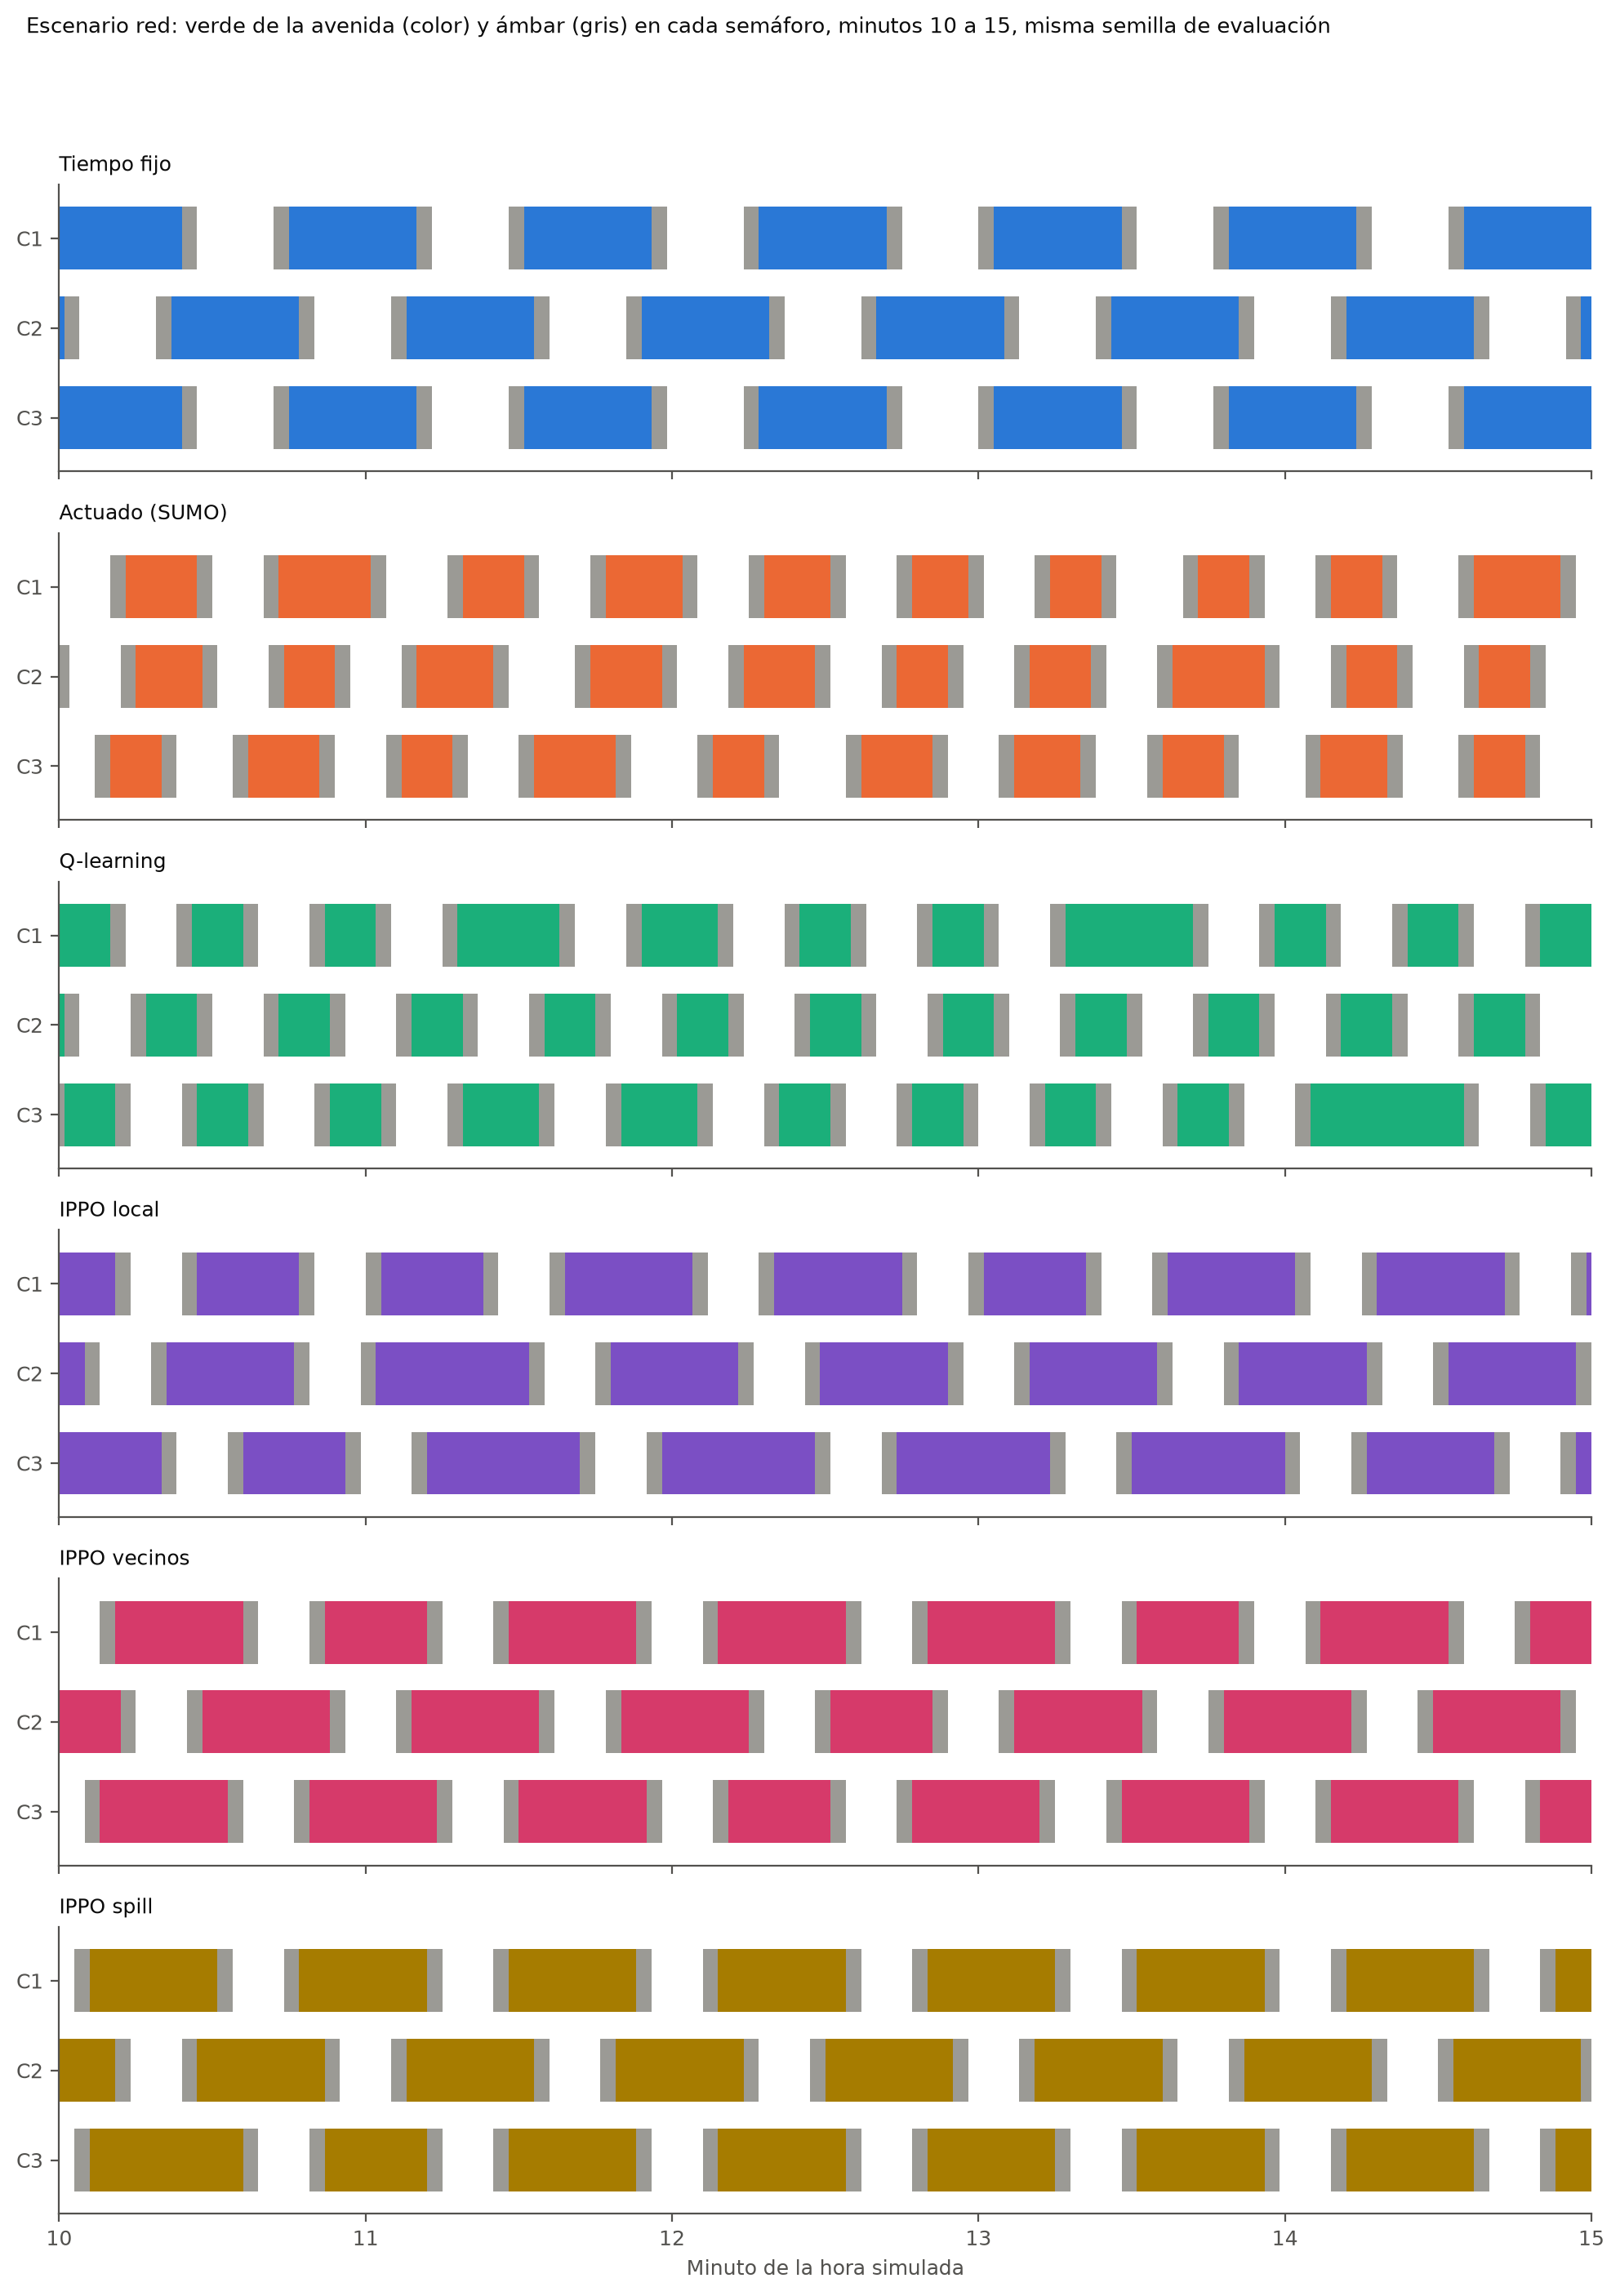
\includegraphics[width=0.90\textwidth]{fig_red_fases.png}
  \caption[Escenario red: verde de la avenida por semáforo]{Escenario red (fase exploratoria): verde de la avenida (en color) y ámbar (en gris) de cada semáforo entre los minutos 10 y 15 de la hora simulada, con la semilla de evaluación 1001, bajo el fijo con onda verde, el actuado, Q-learning y las variantes IPPO (políticas del último episodio); en blanco, el verde de la transversal.}
  \label{fig:red-fases}
\end{figure}
% fuente: graficar.py, figura 7 (ventana de 600 a 900 s; color = fase de la avenida,
% gris = fases impares de ambar); fases_red_<brazo>_s1001.csv de demo_rl

\subsection*{E3-U4: corredor de dos cruces}

En el corredor, \emph{local} iguala al fijo tuneado ($+0.6$\,\%,
$p = 0.58$) y queda un $1.7$\,\% por encima del actuado. Las tres
políticas de \emph{vecinos} (19.84, 19.90 y 20.37~s) superan a las dos
referencias: la mediana da $-6.2$\,\% frente al fijo y $-5.1$\,\% frente
al actuado, con $p = 0.002$ en los dos (Tabla~\ref{tab:corredor-u4}).
Fue el primer control aprendido que superó al actuado en un escenario de
varios cruces, aunque lejos de la meta de $-25$\,\%.

Frente al fijo de la primera ronda, estas mismas políticas mostraban
$-38$\,\% de retraso: la diferencia entre las dos lecturas mide cuánto
pesaba el reparto de verde de la referencia, no lo que hace el agente.
El plan de pruebas confirma la lectura frente al fijo tuneado: en P1,
IPPO vecinos funciona ($-6.8$\,\% frente al fijo y $-5.8$\,\% frente al
actuado) e IPPO local empata con el fijo.
% fuente: plan2/veredicto_congelado_0355.csv (P1: ippo_vecinos delta_fijo -6.8, delta_act -5.8,
% FUNCIONA; ippo_local EMPATA)

El fijo tuneado ya forma una onda verde eficaz: el $91$\,\% de los
vehículos de paso se detiene a lo sumo una vez. \emph{Vecinos} sube esa
fracción a 0.95 (actuado 0.73, Q-learning 0.32), baja el retraso en el
sentido punta de 24 a 20~s y reduce la cola máxima del enlace entre
cruces de 8 a 5.5 vehículos, abriendo la avenida en pelotón de un cruce
al siguiente (Figura~\ref{fig:corredor-fases}). \emph{Local} llega a lo
mismo que el fijo con detectores propios, porque con 300~m entre cruces
el pelotón que sale del primero ya es visible para el segundo en su
propia aproximación.

% Generado por tablas_tex.py a partir de los CSV del proyecto. No editar a mano.
\begin{table}[H]
\setstretch{1}
\centering
\scriptsize
\setlength{\tabcolsep}{3pt}
\setlength{\tabcolsep}{2pt}\begin{tabular}{p{2.8cm}rrrrrr}
\toprule
Métrica & \makecell{Fijo} & \makecell{Actuado} & \makecell{Q-learning} & \makecell{IPPO sin\\mensajes} & \makecell{IPPO con\\mensajes} & \makecell{IPPO con\\penalización} \\
\midrule
Retraso (s/veh) & 21.15 $\pm$ 0.41 & 20.91 $\pm$ 0.25 & 33.86 $\pm$ 1.66 & 21.27 $\pm$ 0.33 & 19.84 $\pm$ 0.36 & 20.21 $\pm$ 0.28 \\
Espera detenida (s/veh) & 6.97 $\pm$ 0.18 & 5.90 $\pm$ 0.14 & 12.27 $\pm$ 0.50 & 7.37 $\pm$ 0.20 & 6.52 $\pm$ 0.23 & 6.77 $\pm$ 0.16 \\
Cola promedio (veh) & 3.81 $\pm$ 0.08 & 3.32 $\pm$ 0.07 & 6.38 $\pm$ 0.23 & 4.01 $\pm$ 0.10 & 3.60 $\pm$ 0.11 & 3.72 $\pm$ 0.08 \\
Cola máxima (veh) & 16.10 $\pm$ 1.52 & 16.70 $\pm$ 1.01 & 22.40 $\pm$ 1.66 & 15.20 $\pm$ 0.56 & 14.10 $\pm$ 0.53 & 14.80 $\pm$ 1.11 \\
Paradas por vehículo & 0.80 $\pm$ 0.02 & 0.83 $\pm$ 0.02 & 1.54 $\pm$ 0.08 & 0.77 $\pm$ 0.02 & 0.67 $\pm$ 0.01 & 0.68 $\pm$ 0.01 \\
Throughput (veh) & 1770 $\pm$ 1 & 1766 $\pm$ 1 & 1758 $\pm$ 4 & 1767 $\pm$ 2 & 1768 $\pm$ 2 & 1768 $\pm$ 2 \\
CO$_2$ (g/veh) & 219.76 $\pm$ 0.82 & 221.59 $\pm$ 0.59 & 244.32 $\pm$ 2.70 & 219.27 $\pm$ 0.75 & 216.27 $\pm$ 0.78 & 217.22 $\pm$ 0.60 \\
NO$_x$ (mg/veh) & 75.59 $\pm$ 0.27 & 75.94 $\pm$ 0.18 & 83.81 $\pm$ 0.92 & 75.52 $\pm$ 0.27 & 74.49 $\pm$ 0.27 & 74.79 $\pm$ 0.21 \\
Recompensa por decisión & $-$1.87 $\pm$ 0.04 & $-$1.58 $\pm$ 0.04 & $-$3.22 $\pm$ 0.12 & $-$1.99 $\pm$ 0.06 & $-$1.76 $\pm$ 0.06 & $-$1.83 $\pm$ 0.05 \\
Cambios de fase & 410.40 $\pm$ 0.37 & 459.30 $\pm$ 4.17 & 462.70 $\pm$ 3.04 & 369.10 $\pm$ 2.12 & 371.60 $\pm$ 1.02 & 366.90 $\pm$ 1.45 \\
Viaje extremo a extremo (s) & 105.82 $\pm$ 0.82 & 108.22 $\pm$ 0.50 & 131.81 $\pm$ 2.89 & 104.55 $\pm$ 0.40 & 102.35 $\pm$ 0.42 & 102.23 $\pm$ 0.53 \\
Retraso extremo a extremo (s) & 22.88 $\pm$ 0.77 & 25.27 $\pm$ 0.44 & 48.87 $\pm$ 2.89 & 21.61 $\pm$ 0.37 & 19.42 $\pm$ 0.38 & 19.29 $\pm$ 0.48 \\
Tasa de \textit{spillback} & 0.00 $\pm$ 0.00 & 0.00 $\pm$ 0.00 & 0.00 $\pm$ 0.00 & 0.00 $\pm$ 0.00 & 0.00 $\pm$ 0.00 & 0.00 $\pm$ 0.00 \\
Cola máxima en un enlace (veh) & 7.90 $\pm$ 0.92 & 7.20 $\pm$ 0.45 & 10.90 $\pm$ 1.09 & 6.50 $\pm$ 0.61 & 5.50 $\pm$ 1.23 & 5.40 $\pm$ 0.84 \\
Retraso de paso, sentido punta (s) & 24.39 $\pm$ 1.16 & 26.49 $\pm$ 0.56 & 58.01 $\pm$ 4.02 & 22.89 $\pm$ 0.53 & 20.34 $\pm$ 0.45 & 20.13 $\pm$ 0.53 \\
Paradas de paso (/veh) & 0.81 $\pm$ 0.04 & 1.00 $\pm$ 0.03 & 2.24 $\pm$ 0.14 & 0.77 $\pm$ 0.03 & 0.60 $\pm$ 0.02 & 0.59 $\pm$ 0.02 \\
Fracción de paso con $\le 1$ parada & 0.91 $\pm$ 0.01 & 0.73 $\pm$ 0.02 & 0.32 $\pm$ 0.01 & 0.90 $\pm$ 0.01 & 0.95 $\pm$ 0.01 & 0.95 $\pm$ 0.01 \\
Segundos con \textit{spillback} & 0 $\pm$ 0 & 0 $\pm$ 0 & 0 $\pm$ 0 & 0 $\pm$ 0 & 0 $\pm$ 0 & 0 $\pm$ 0 \\
Vehículos máximos en un enlace & 14.60 $\pm$ 1.48 & 12.30 $\pm$ 0.59 & 24.20 $\pm$ 2.69 & 11.80 $\pm$ 0.56 & 11.80 $\pm$ 0.66 & 11.20 $\pm$ 0.74 \\
Vehículos no terminados & 0 $\pm$ 0 & 0 $\pm$ 0 & 0 $\pm$ 0 & 0 $\pm$ 0 & 0 $\pm$ 0 & 0 $\pm$ 0 \\
\bottomrule
\end{tabular}
\caption[Escenario corredor: evaluación de las variantes IPPO]{Escenario corredor: evaluación con política congelada sobre 10 semillas (1001 a 1010), las mismas para todos los brazos; media $\pm$ IC95\,\%. Cada variante IPPO es la política mediana de sus semillas base por la evaluación intermedia final; los cambios porcentuales están en la Tabla~\ref{tab:corredor-u4-deltas}.}
\label{tab:corredor-u4}
\end{table}
\begin{table}[H]
\setstretch{1}
\centering
\scriptsize
\setlength{\tabcolsep}{3pt}
\begin{tabular}{lrrrrrrr}
\toprule
 & Retraso & \multicolumn{3}{c}{Cambio del retraso [IC95\,\%]} & \multicolumn{3}{c}{vs fijo, secundarias} \\
\cmidrule(lr){3-5}\cmidrule(lr){6-8}
Variante & (s/veh) & vs fijo & vs actuado & vs Q-learning & Espera & Paradas & Cambios \\
\midrule
IPPO sin mensajes & 21.27 & \makecell[r]{+0.6\,\%\\{}[$-$1.1, 2.2]\\$p$ = 0.576} & \makecell[r]{+1.7\,\%\\{}[0.2, 3.3]\\$p$ = 0.125} & \makecell[r]{$-$37.2\,\%\\{}[$-$40.1, $-$34.1]\\$p$ = 0.00195} & +5.7\,\% & $-$2.8\,\% & $-$10.1\,\% \\
IPPO con mensajes & 19.84 & \makecell[r]{$-$6.2\,\%\\{}[$-$8.0, $-$4.6]\\$p$ = 0.00195} & \makecell[r]{$-$5.1\,\%\\{}[$-$6.4, $-$3.9]\\$p$ = 0.00195} & \makecell[r]{$-$41.4\,\%\\{}[$-$43.8, $-$39.0]\\$p$ = 0.00195} & $-$6.5\,\% & $-$15.9\,\% & $-$9.5\,\% \\
IPPO con penalización & 20.21 & \makecell[r]{$-$4.4\,\%\\{}[$-$5.7, $-$3.1]\\$p$ = 0.00195} & \makecell[r]{$-$3.3\,\%\\{}[$-$4.8, $-$2.0]\\$p$ = 0.00391} & \makecell[r]{$-$40.3\,\%\\{}[$-$42.9, $-$37.6]\\$p$ = 0.00195} & $-$3.0\,\% & $-$15.1\,\% & $-$10.6\,\% \\
\bottomrule
\end{tabular}
\caption[Escenario corredor: cambio del retraso de las variantes IPPO]{Escenario corredor: cambio porcentual del retraso de cada variante IPPO (política mediana) frente al fijo, al actuado y a Q-learning, con intervalo bootstrap pareado por semilla y $p$ de Wilcoxon pareado; a la derecha, cambio frente al fijo de tres secundarias.}
\label{tab:corredor-u4-deltas}
\end{table}


\begin{figure}[H]
  \centering
  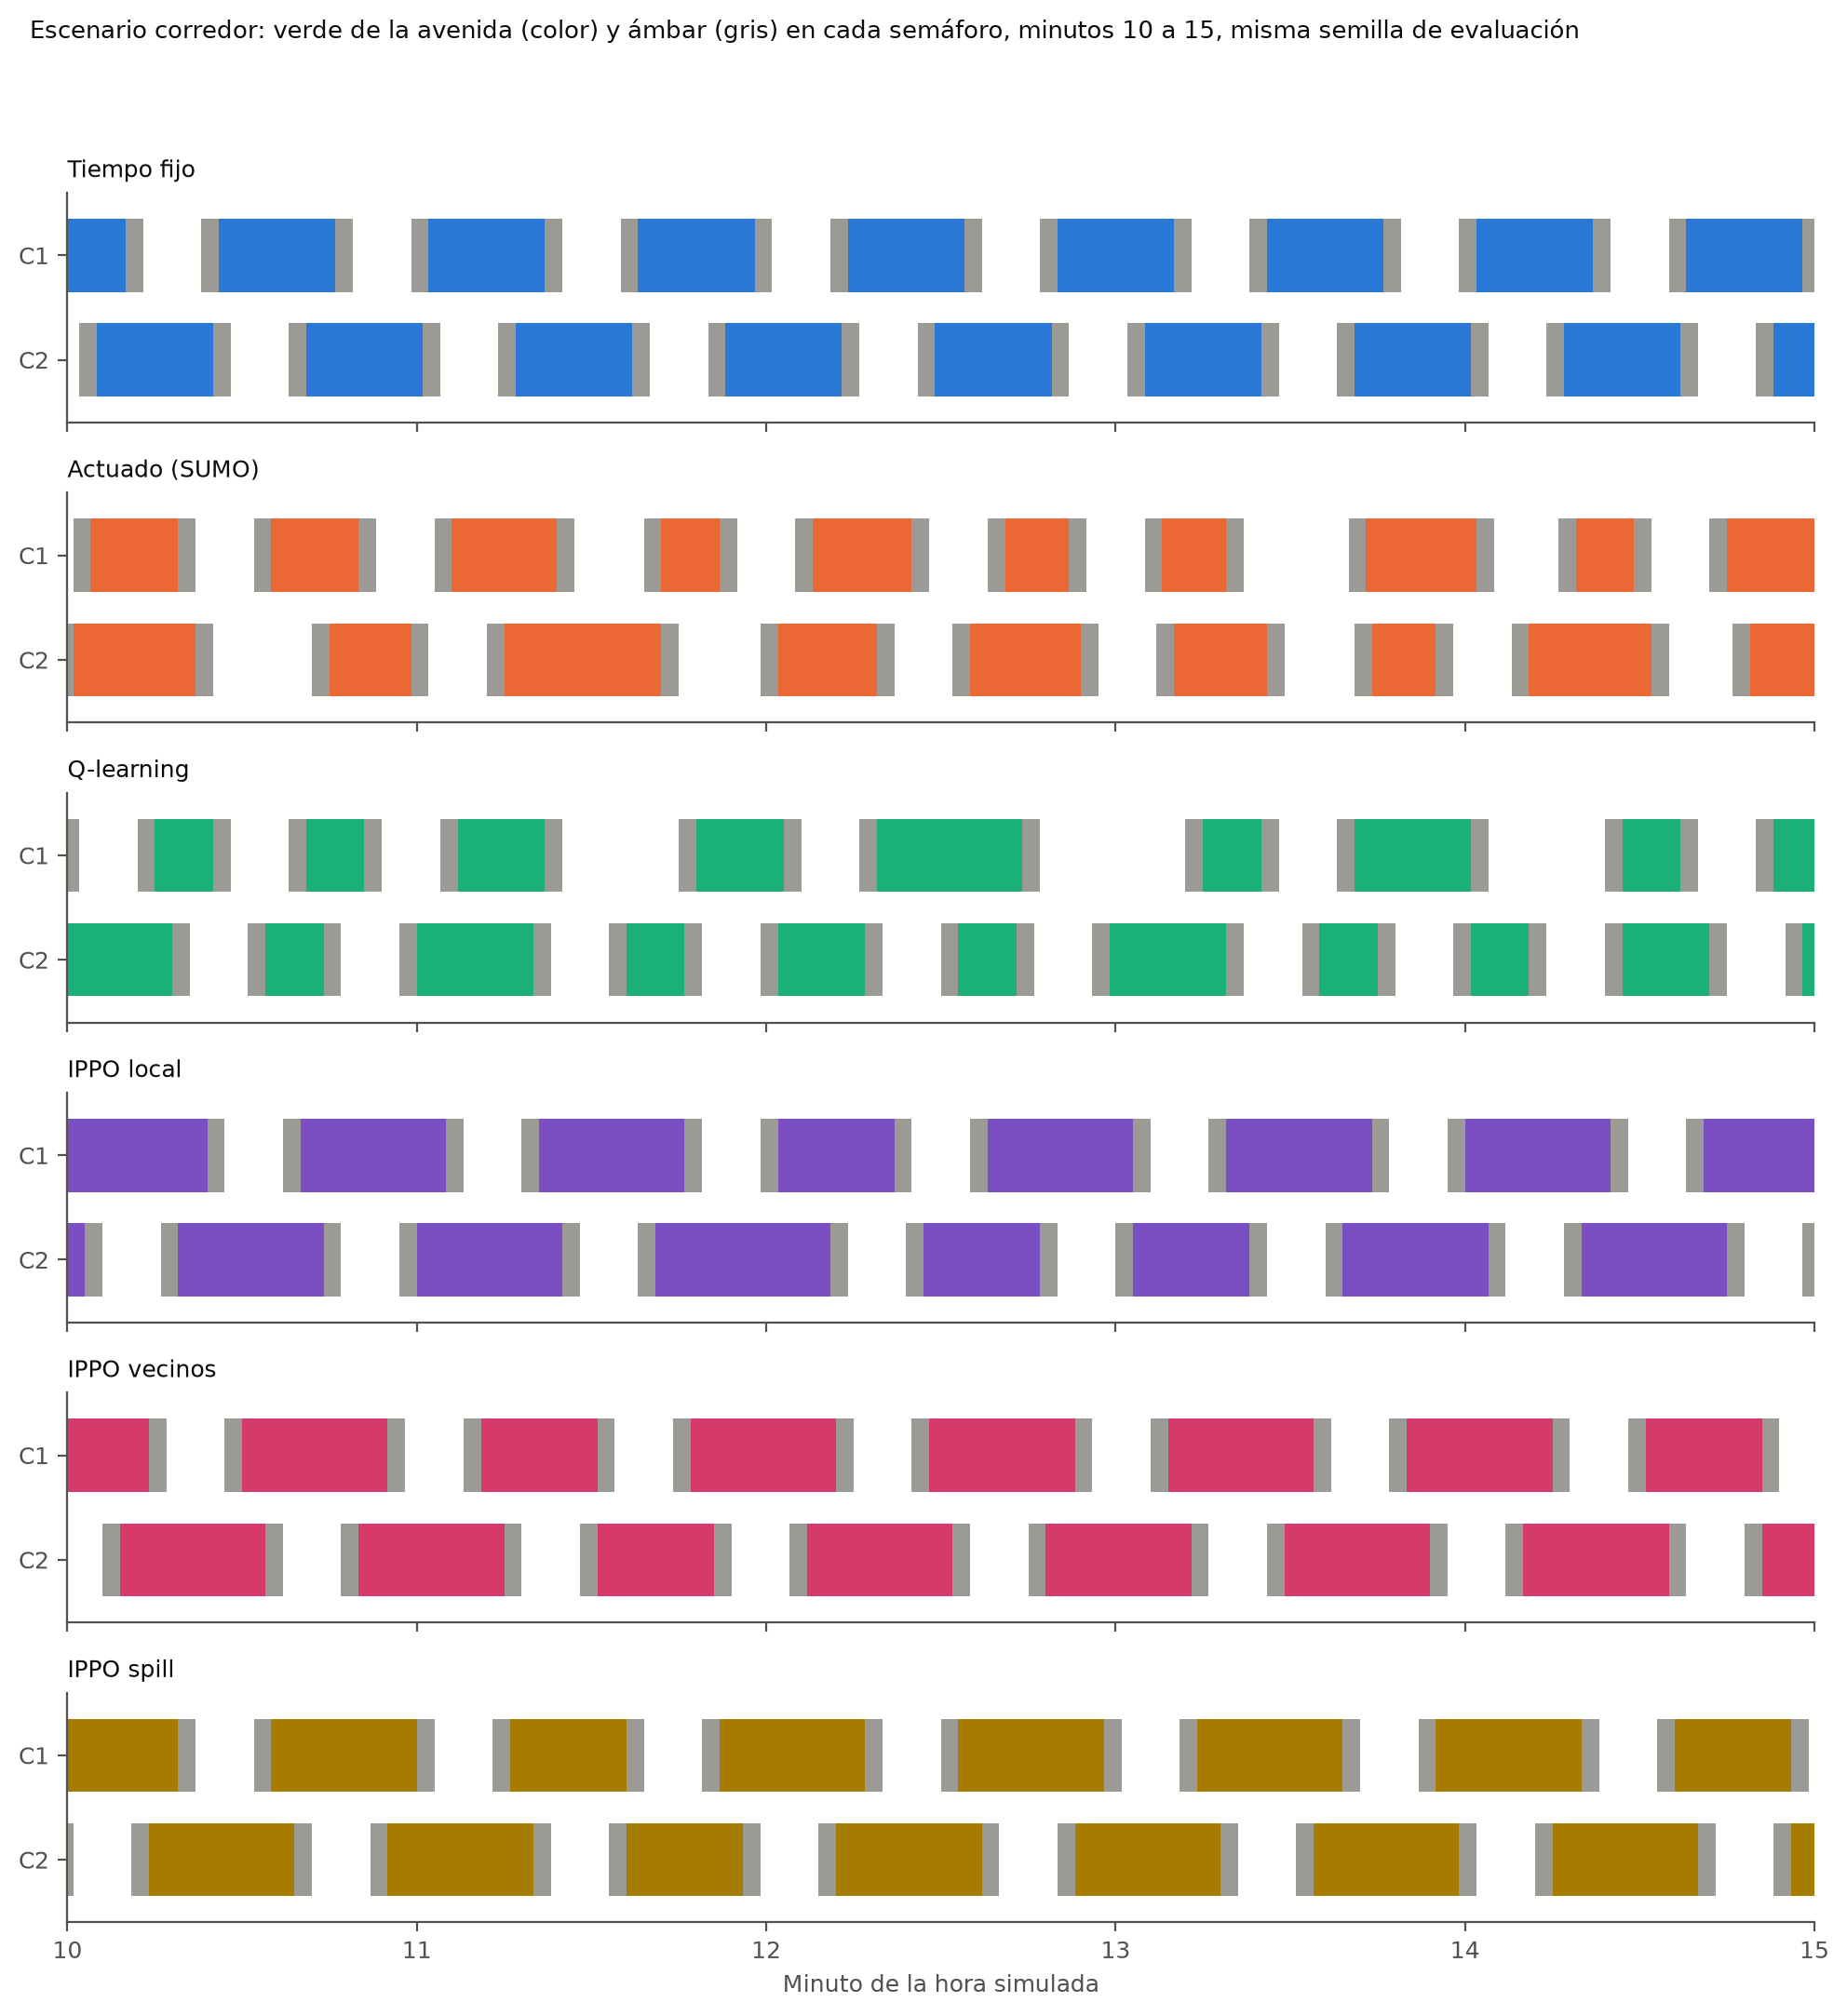
\includegraphics[width=0.90\textwidth]{fig_corredor_fases.png}
  \caption[Escenario corredor: verde de la avenida por semáforo]{Escenario corredor (fase exploratoria): verde de la avenida (en color) y ámbar (en gris) de cada semáforo entre los minutos 10 y 15 de la hora simulada, con la semilla de evaluación 1001, bajo cada control (políticas IPPO del último episodio); en blanco, el verde de la transversal.}
  \label{fig:corredor-fases}
\end{figure}
% fuente: graficar.py, figura 7; fases_corredor_<brazo>_s1001.csv de demo_rl

\subsection*{E6: corredor con demanda doble}

Con la demanda del corredor multiplicada por dos (3620 vehículos en la
hora) ningún control evita la saturación. El fijo tuneado para esta
demanda deja 154~s de retraso por vehículo, el actuado 123~s y el agente
tabular 211~s; este es el único que deja vehículos sin terminar a los
6000 pasos en algunas semillas (Tabla~\ref{tab:corredor_alta-u4}).
\emph{Vecinos} y \emph{spill} se entrenaron con tres semillas base y
\emph{local} con una. Las medianas (122.0~s en \emph{local}, 121.3~s en
\emph{vecinos} y 122.8~s en \emph{spill}) quedan entre un $-20$ y un
$-21$\,\% del fijo (las siete políticas, entre $-20$ y $-23$\,\%), y
frente al actuado sus intervalos incluyen el cero: en esta fase lo
igualaban.

El plan de pruebas cambió esta lectura, para IPPO y para el agente
tabular. En P2, con la política elegida por validación, las tres
variantes IPPO superan al actuado, e IPPO vecinos queda un $4.4$\,\%
por debajo de él (intervalo $-6.3$ a $-2.6$\,\%), con veredicto
FUNCIONA. Q-learning, con la recompensa de retraso y el protocolo del
plan, mejora al fijo un $8.8$\,\% (veredicto MEJORA) sin dejar
vehículos sin terminar, aunque queda un $13.7$\,\% por detrás del
actuado.
% fuente: plan2/veredicto_congelado_0355.csv (P2, ippo_vecinos: delta_act -4.4 [-6.3, -2.6], FUNCIONA;
% ql: delta_fijo -8.8 [-9.9, -7.5], delta_act 13.7, MEJORA); vehiculos sin terminar: texto original
% (git show 7bd8685:TESIS/secciones/conclusiones.tex, conclusion 7); medianas y politicas:
% tablas/corredor_alta_u4.tex y tablas/corredor_alta_fragilidad.tex

El análisis de robustez matiza esta lectura (Sección~\ref{sec:robustez}).
En P2 la espera para entrar a la red es mayor que el
\texttt{timeLoss}. La política publicada de IPPO vecinos baja el
\texttt{timeLoss} un $23.3$\,\% frente al fijo, pero su espera para
entrar sube de 240 a 282~s/veh, y con el retraso total queda un
$1.6$\,\% por encima del fijo.
% fuente: plan2/evaluacion_corredor_alta_resumen.csv (fijo: timeloss_prom 154.70, retraso_insercion_prom
% 239.57; ippo_vecinos_s2042: timeloss_prom delta_pct -23.3, retraso_insercion_prom 282.02);
% plan2/robustez_veredicto.csv (P2, ippo_vecinos: delta_fijo +1.6, FALLA); hechos_v21.md

La meta de \textit{throughput}, la única que este escenario permite
evaluar, no está al alcance de ningún control. Las siete políticas IPPO
completan entre 2914 y 2938 viajes en la hora, un 2 a 3\,\% más que el
actuado (2852) y lo mismo que el fijo (2923): la demanda supera la
capacidad del carril y los controles sirven el máximo que la geometría
admite. En los escenarios nominales la meta tampoco es evaluable: todos
los vehículos terminan su viaje bajo los tres controles y solo entre un
2 y un 3\,\% llega después de los 3600~s.

El actuado llena el carril del enlace entre los dos cruces en las diez
semillas (38 vehículos, la capacidad) y pasa 79~s de la hora en
\textit{spillback}. En promedio sobre las diez semillas, las siete
políticas IPPO mantienen la cola máxima del enlace entre 31 y 33
vehículos, bajo el umbral de 34 que define el \textit{spillback}
(Sección~\ref{sec:u3}), y acumulan entre 0 y 3~s de
\textit{spillback}; en algunas semillas llegan al umbral o lo pasan. La
Figura~\ref{fig:corredor-alta-spillback} muestra las políticas medianas
de cada variante.
% fuente: evaluacion_corredor_alta.csv de demo_rl (cola_max_enlace y spillback_seg por brazo y
% semilla: medias de 31.1 a 32.6 veh y de 0 a 2.9 s; maximos de 34 a 37 veh en ippo_local,
% ippo_vecinos_s42 e ippo_spill_s42|s2042|s4042); graficar.py, figura 8 (brazos IPPO = politica mediana)

\emph{Spill} no reduce la cola del enlace frente a \emph{vecinos}
(31.9 contra 31.1 vehículos en sus políticas medianas): cuando la
mensajería ya lleva al agente la cola del enlace, la penalización es
redundante. Con la avenida saturada en los dos sentidos no hay onda
verde posible, y la ventaja de IPPO en este escenario es de gestión de
colas, no de coordinación de fases.

% Generado por tablas_tex.py a partir de los CSV del proyecto. No editar a mano.
\begin{table}[H]
\setstretch{1}
\centering
\scriptsize
\setlength{\tabcolsep}{3pt}
\setlength{\tabcolsep}{2pt}\begin{tabular}{p{2.8cm}rrrrrr}
\toprule
Métrica & \makecell{Fijo} & \makecell{Actuado} & \makecell{Q-learning} & \makecell{IPPO sin\\mensajes} & \makecell{IPPO con\\mensajes} & \makecell{IPPO con\\penalización} \\
\midrule
Retraso (s/veh) & 153.88 $\pm$ 2.15 & 122.97 $\pm$ 3.69 & 211.12 $\pm$ 22.60 & 121.97 $\pm$ 1.23 & 121.33 $\pm$ 1.53 & 122.78 $\pm$ 2.09 \\
Espera detenida (s/veh) & 62.59 $\pm$ 1.24 & 74.82 $\pm$ 3.23 & 88.28 $\pm$ 25.04 & 64.00 $\pm$ 1.39 & 64.80 $\pm$ 1.25 & 63.91 $\pm$ 2.04 \\
Cola promedio (veh) & 44.54 $\pm$ 0.77 & 49.57 $\pm$ 2.09 & 55.17 $\pm$ 15.08 & 44.02 $\pm$ 0.83 & 44.27 $\pm$ 0.82 & 43.57 $\pm$ 1.19 \\
Cola máxima (veh) & 105.90 $\pm$ 4.03 & 151.70 $\pm$ 10.51 & 158.40 $\pm$ 23.43 & 127.90 $\pm$ 5.17 & 134.70 $\pm$ 6.38 & 133.10 $\pm$ 8.53 \\
Paradas por vehículo & 6.29 $\pm$ 0.09 & 2.87 $\pm$ 0.07 & 7.30 $\pm$ 0.27 & 3.73 $\pm$ 0.04 & 3.58 $\pm$ 0.08 & 3.76 $\pm$ 0.02 \\
Throughput (veh) & 2923 $\pm$ 7 & 2852 $\pm$ 16 & 2667 $\pm$ 77 & 2928 $\pm$ 8 & 2918 $\pm$ 7 & 2914 $\pm$ 11 \\
CO$_2$ (g/veh) & 432.43 $\pm$ 3.17 & 387.27 $\pm$ 5.68 & 507.07 $\pm$ 35.23 & 385.00 $\pm$ 1.87 & 383.94 $\pm$ 2.29 & 385.93 $\pm$ 3.12 \\
NO$_x$ (mg/veh) & 151.39 $\pm$ 1.24 & 137.48 $\pm$ 2.25 & 179.09 $\pm$ 14.30 & 135.60 $\pm$ 0.76 & 135.36 $\pm$ 0.88 & 135.93 $\pm$ 1.27 \\
Recompensa por decisión & $-$23.89 $\pm$ 0.43 & $-$30.60 $\pm$ 1.61 & $-$31.80 $\pm$ 9.77 & $-$25.16 $\pm$ 0.58 & $-$25.46 $\pm$ 0.57 & $-$24.84 $\pm$ 0.89 \\
Cambios de fase & 446.80 $\pm$ 1.65 & 261.40 $\pm$ 3.43 & 590.80 $\pm$ 51.34 & 300.50 $\pm$ 2.17 & 277.60 $\pm$ 1.36 & 302.80 $\pm$ 3.89 \\
Viaje extremo a extremo (s) & 265.67 $\pm$ 3.17 & 257.63 $\pm$ 2.05 & 320.79 $\pm$ 18.46 & 258.52 $\pm$ 1.60 & 257.19 $\pm$ 1.85 & 258.14 $\pm$ 1.61 \\
Retraso extremo a extremo (s) & 182.75 $\pm$ 3.19 & 174.72 $\pm$ 2.01 & 238.14 $\pm$ 18.69 & 175.61 $\pm$ 1.60 & 174.27 $\pm$ 1.82 & 175.23 $\pm$ 1.63 \\
Tasa de \textit{spillback} & 0.00 $\pm$ 0.00 & 0.02 $\pm$ 0.01 & 0.00 $\pm$ 0.00 & 0.00 $\pm$ 0.00 & 0.00 $\pm$ 0.00 & 0.00 $\pm$ 0.00 \\
Cola máxima en un enlace (veh) & 23.80 $\pm$ 0.66 & 38.00 $\pm$ 0.00 & 33.70 $\pm$ 2.63 & 31.70 $\pm$ 1.47 & 31.10 $\pm$ 0.92 & 31.90 $\pm$ 1.09 \\
Retraso de paso, sentido punta (s) & 191.41 $\pm$ 4.47 & 190.99 $\pm$ 2.66 & 279.93 $\pm$ 20.40 & 191.32 $\pm$ 1.64 & 189.30 $\pm$ 1.83 & 193.71 $\pm$ 1.66 \\
Paradas de paso (/veh) & 8.10 $\pm$ 0.15 & 4.11 $\pm$ 0.12 & 9.09 $\pm$ 0.89 & 5.47 $\pm$ 0.10 & 5.24 $\pm$ 0.11 & 5.48 $\pm$ 0.07 \\
Fracción de paso con $\le 1$ parada & 0.16 $\pm$ 0.00 & 0.30 $\pm$ 0.02 & 0.07 $\pm$ 0.02 & 0.22 $\pm$ 0.02 & 0.24 $\pm$ 0.01 & 0.25 $\pm$ 0.02 \\
Segundos con \textit{spillback} & 0 $\pm$ 0 & 79 $\pm$ 29 & 29 $\pm$ 46 & 2 $\pm$ 4 & 0 $\pm$ 0 & 0 $\pm$ 0 \\
Vehículos máximos en un enlace & 37.00 $\pm$ 0.00 & 38.00 $\pm$ 0.00 & 37.30 $\pm$ 0.35 & 37.20 $\pm$ 0.30 & 37.30 $\pm$ 0.35 & 37.30 $\pm$ 0.35 \\
Vehículos no terminados & 0 $\pm$ 0 & 0 $\pm$ 0 & 9 $\pm$ 19 & 0 $\pm$ 0 & 0 $\pm$ 0 & 0 $\pm$ 0 \\
\bottomrule
\end{tabular}
\caption[Escenario corredor\_alta: evaluación de las variantes IPPO]{Escenario corredor\_alta: evaluación con política congelada sobre 10 semillas (1001 a 1010), las mismas para todos los brazos; media $\pm$ IC95\,\%. Cada variante IPPO es la política mediana de sus semillas base por la evaluación intermedia final; los cambios porcentuales están en la Tabla~\ref{tab:corredor_alta-u4-deltas}.}
\label{tab:corredor_alta-u4}
\end{table}
\begin{table}[H]
\setstretch{1}
\centering
\scriptsize
\setlength{\tabcolsep}{3pt}
\begin{tabular}{lrrrrrrr}
\toprule
 & Retraso & \multicolumn{3}{c}{Cambio del retraso [IC95\,\%]} & \multicolumn{3}{c}{vs fijo, secundarias} \\
\cmidrule(lr){3-5}\cmidrule(lr){6-8}
Variante & (s/veh) & vs fijo & vs actuado & vs Q-learning & Espera & Paradas & Cambios \\
\midrule
IPPO sin mensajes & 121.97 & \makecell[r]{$-$20.7\,\%\\{}[$-$21.8, $-$19.5]\\$p$ = 0.00195} & \makecell[r]{$-$0.8\,\%\\{}[$-$3.0, 1.6]\\$p$ = 0.695} & \makecell[r]{$-$42.2\,\%\\{}[$-$47.1, $-$36.9]\\$p$ = 0.00195} & +2.2\,\% & $-$40.7\,\% & $-$32.7\,\% \\
IPPO con mensajes & 121.33 & \makecell[r]{$-$21.2\,\%\\{}[$-$22.2, $-$20.0]\\$p$ = 0.00195} & \makecell[r]{$-$1.3\,\%\\{}[$-$3.8, 1.4]\\$p$ = 0.334} & \makecell[r]{$-$42.5\,\%\\{}[$-$47.6, $-$37.1]\\$p$ = 0.00195} & +3.5\,\% & $-$43.2\,\% & $-$37.9\,\% \\
IPPO con penalización & 122.78 & \makecell[r]{$-$20.2\,\%\\{}[$-$21.7, $-$18.4]\\$p$ = 0.00195} & \makecell[r]{$-$0.2\,\%\\{}[$-$3.2, 3.5]\\$p$ = 0.922} & \makecell[r]{$-$41.8\,\%\\{}[$-$47.0, $-$36.3]\\$p$ = 0.00195} & +2.1\,\% & $-$40.2\,\% & $-$32.2\,\% \\
\bottomrule
\end{tabular}
\caption[Escenario corredor\_alta: cambio del retraso de las variantes IPPO]{Escenario corredor\_alta: cambio porcentual del retraso de cada variante IPPO (política mediana) frente al fijo, al actuado y a Q-learning, con intervalo bootstrap pareado por semilla y $p$ de Wilcoxon pareado; a la derecha, cambio frente al fijo de tres secundarias.}
\label{tab:corredor_alta-u4-deltas}
\end{table}


\begin{figure}[H]
  \centering
  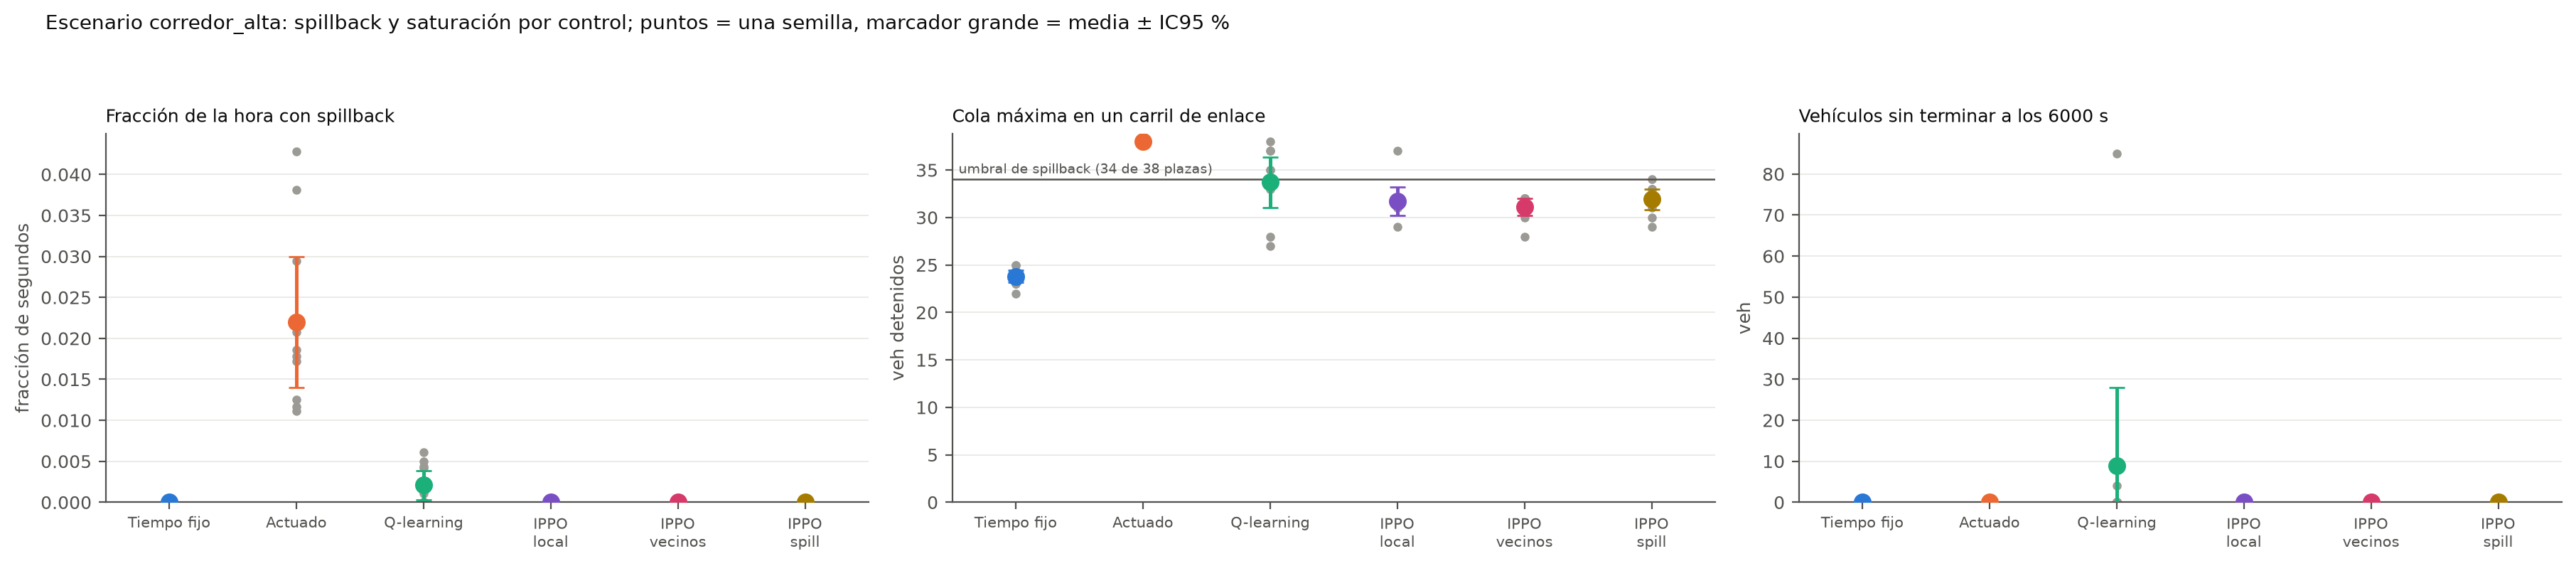
\includegraphics[width=0.95\textwidth]{fig_corredor_alta_spillback.png}
  \caption[Escenario corredor\_alta: \textit{spillback} y saturación]{Escenario corredor\_alta (fase exploratoria): fracción de la hora con \textit{spillback}, cola máxima en un carril del enlace y vehículos sin terminar, por control. Cada punto gris es una semilla de evaluación y el marcador grande es la media con su IC95\,\%; la línea horizontal del panel central marca el umbral de \textit{spillback} (34 de 38 plazas).}
  \label{fig:corredor-alta-spillback}
\end{figure}
% fuente: graficar.py, figura 8

\subsection*{Canal de mensajes imperfecto}

La política mediana de \emph{vecinos}, entrenada con mensajes
instantáneos, se evaluó sin reentrenar con latencia y pérdida de
mensajes (Tablas~\ref{tab:red-s1} y~\ref{tab:corredor-s1}). Es la única
prueba de robustez al canal del documento; el plan de pruebas no la
repitió.

En la red, con latencia de 5~s y pérdida del 30\,\% la política pierde
0.8~s frente al canal perfecto y queda un $4$\,\% por detrás del fijo
tuneado; con latencia de 10~s pierde 2.2~s y queda un $10$\,\% por
detrás. Con latencia de 5~s sin pérdida el retraso global incluso baja,
a 21.19~s, pero con más cambios de fase y menos progresión, como el
actuado.

% Generado por tablas_tex.py a partir de los CSV del proyecto. No editar a mano.
\begin{table}[H]
\setstretch{1}
\centering
\scriptsize
\setlength{\tabcolsep}{3pt}
\begin{tabular}{lrrrrr}
\toprule
Canal & Retraso (s/veh) & \makecell{Diferencia vs\\perfecto (s)} & \makecell{Paso con\\$\le 1$ parada} & \makecell{Retraso de paso\\punta (s)} & Cambios \\
\midrule
canal perfecto & 21.89 $\pm$ 0.28 & -- & 0.985 & 23.6 & 569.5 \\
latencia 5~s & 21.19 $\pm$ 0.26 & $-$0.70 $\pm$ 0.26 & 0.795 & 27.7 & 791.7 \\
latencia 5~s, pérdida 30\,\% & 22.70 $\pm$ 0.23 & +0.81 $\pm$ 0.31 & 0.705 & 29.7 & 753.6 \\
latencia 10~s & 24.04 $\pm$ 0.12 & +2.16 $\pm$ 0.27 & 0.542 & 32.7 & 734.4 \\
\bottomrule
\end{tabular}
\caption[Escenario red: IPPO con mensajes y canal imperfecto]{Escenario red: la política mediana de IPPO con mensajes evaluada con latencia y pérdida de mensajes, sin reentrenar, sobre las mismas semillas. La diferencia frente al canal perfecto es la media pareada por semilla $\pm$ IC95\,\%.}
\label{tab:red-s1}
\end{table}


En el corredor la política pierde 1.4~s con latencia de 5~s, 2.2~s con
latencia de 5~s y pérdida del 30\,\% y 2.5~s con latencia de 10~s. Con
el primer canal empata con el fijo tuneado ($+0.6$\,\%, intervalo
$-1.0$ a $+2.2$\,\%); con los otros dos queda por encima de él ($+4.2$ y
$+5.8$\,\%), y frente al actuado queda por encima en los tres ($+1.7$,
$+5.4$ y $+7.0$\,\%). Pierde así la ventaja que tenía frente a las dos
referencias.
% fuente: evaluacion_corredor_resumen.csv de demo_rl, brazos ippo_vecinos_L5p0, _L5p30 y _L10p0
% (timeloss_prom: delta_pct 0.6 [-1.0, 2.2], 4.2 y 5.8; delta_pct_act 1.7, 5.4 y 7.0)

% Generado por tablas_tex.py a partir de los CSV del proyecto. No editar a mano.
\begin{table}[H]
\setstretch{1}
\centering
\scriptsize
\setlength{\tabcolsep}{3pt}
\begin{tabular}{lrrrrr}
\toprule
Canal & Retraso (s/veh) & \makecell{Diferencia vs\\perfecto (s)} & \makecell{Paso con\\$\le 1$ parada} & \makecell{Retraso de paso\\punta (s)} & Cambios \\
\midrule
canal perfecto & 19.84 $\pm$ 0.36 & -- & 0.952 & 20.3 & 371.6 \\
latencia 5~s & 21.27 $\pm$ 0.20 & +1.44 $\pm$ 0.26 & 0.853 & 24.0 & 414.1 \\
latencia 5~s, pérdida 30\,\% & 22.04 $\pm$ 0.21 & +2.20 $\pm$ 0.53 & 0.774 & 26.4 & 429.0 \\
latencia 10~s & 22.38 $\pm$ 0.41 & +2.54 $\pm$ 0.51 & 0.646 & 28.5 & 448.4 \\
\bottomrule
\end{tabular}
\caption[Escenario corredor: IPPO con mensajes y canal imperfecto]{Escenario corredor: la política mediana de IPPO con mensajes evaluada con latencia y pérdida de mensajes, sin reentrenar, sobre las mismas semillas. La diferencia frente al canal perfecto es la media pareada por semilla $\pm$ IC95\,\%.}
\label{tab:corredor-s1}
\end{table}


En los dos escenarios, cualquier canal imperfecto deshace la
progresión: la fracción de vehículos de paso que se detiene a lo sumo
una vez baja de 0.985 a entre 0.54 y 0.80 en la red, y de 0.95 a entre
0.65 y 0.85 en el corredor. La lectura es que el agente usa el mensaje
del vecino tal cual, sin descontarlo por su edad, porque durante el
entrenamiento nunca vio un mensaje viejo: la edad del mensaje está en la
observación (Tabla~\ref{tab:obs-u4}), pero fuera del rango entrenado no
informa. Entrenar con latencia variable queda en las recomendaciones.
